\documentclass[t,
10pt,
handout, % comment out for getting non handout version
]{beamer}

%beamer settings
\setbeamerfont{normal text}{size=\large}
\AtBeginDocument{\usebeamerfont{normal text}}

% general language
\usepackage{polyglossia}
\setmainfont{Arial}
\setdefaultlanguage{english}
%\usepackage[utf8]{inputenc} % ignor1 anyway due to uft8 based engines
\usepackage[autostyle=true]{csquotes}
\setcounter{tocdepth}{3}
\renewcommand{\baselinestretch}{1.0}

%colors
\usepackage{xcolor}
\definecolor{bluei}{rgb}{0.0, 0.0, 1.0}
\definecolor{greni}{rgb}{0.3, 0.8, 0.2}
\definecolor{greyi}{rgb}{0.5, 0.5 0.5}
\definecolor{b1}{rgb}{0, 0, 0}
\definecolor{r1}{rgb}{255, 0, 0}
\definecolor{green1}{rgb}{0.0, 0.7, 0.0}

% graphics
\usepackage{amssymb}
\usepackage{graphicx}
\usepackage{subcaption}

%date
\usepackage[nodayofweek,level]{datetime}

%change
\newcommand{\authorName}{Janis Jacobi\\ \newline supervisor: Prof. Dr. Niels Schröter}
\newcommand{\topicName}{physics modelling agent}
\newdate{date1}{24}{12}{2025}

% general layout settings for beamer
\usetheme{Madrid}
%\usecolortheme[RGB={0, 100, 250}]{beamer color theme}
\usecolortheme{seahorse}
%\usefonttheme{structurebold}

\useoutertheme{default}
% beamer template
\setbeamercolor{footline left}{bg=blue!20, fg=b1}
\setbeamercolor{footline center}{bg=blue!10, fg=b1}
\setbeamercolor{footline right}{bg=blue!20, fg=b1}
\setbeamertemplate{footline}{%
	\leavevmode%
	\hbox{%
		\begin{beamercolorbox}[wd=.33\paperwidth,ht=2.5ex,dp=1ex,left]{footline left}%
			\hspace{1em}\topicName
		\end{beamercolorbox}%
		\begin{beamercolorbox}[wd=.34\paperwidth,ht=2.5ex,dp=1ex,center]{footline center}%
			\insertshortdate{}
		\end{beamercolorbox}%
		\begin{beamercolorbox}[wd=.33\paperwidth,ht=2.5ex,dp=1ex,right]{footline right}%
			\insertframenumber{} / \inserttotalframenumber\hspace{1em}
		\end{beamercolorbox}%
	}%
}

\setbeamertemplate{headline}{}
% restore visible bullets



% title-page settings
\title{\topicName}
\subtitle{progress report}
\date{\today}
%\logo{logo text}
\author{Janis Jacobi \\ \vspace{1em} supervisor 1: Prof. Dr. Niels Schröter \\ supervisor 2: Prof. Dr. Samir Lounis}

\usepackage[backend=biber, style=numeric, citestyle=numeric, hyperref=true, date=short, backref=false]{biblatex}
%\bibliography{biblio/jabRef.bib}
%\addbibresource{/biblio/jabRef.bib}
\setlength\bibitemsep{7pt}
\setcounter{biburllcpenalty}{9000}

%captions
\usepackage{caption}
\usepackage{subcaption}

%math
\usepackage{mathtools}
\usepackage{unicode-math}
\setmathfont{Latin Modern Math}
\usepackage{amsmath,amssymb}
\usepackage[locale=DE, separate-uncertainty=true]{siunitx}
\usepackage{nicefrac}
\usepackage{siunitx}
\usepackage{physics}
\newcommand{\RNum}[1]{\uppercase\expandafter{\romannumeral #1\relax}} %roman numeral
\numberwithin{equation}{section}
\usepackage{numprint}
\usepackage[version=4]{mhchem}

\newcommand{\al}{\ensuremath{\mathcolor{c1}{|}}}
\newcommand{\scProd}[2]{\ensuremath{\langle #1,#2 \rangle}}
\newcommand{\parti}[2]{\ensuremath{\frac{\mathrm{d}#1}{\mathrm{d}#2}}}
\newcommand{\pard}[2]{\ensuremath{\frac{\partial #1}{\partial #2}}}

% graphics
\usepackage{graphicx}
%\usepackage[margin=2cm]{geometry}
\usepackage{subcaption}
\captionsetup{compatibility=false}

%circuits and drawing
\usepackage{tikz}
\usetikzlibrary{
	shapes.geometric,
	arrows.meta,
	positioning,
	fit,
	calc
}

% insert documents
\usepackage{pdfpages}
\usepackage{float}

% tables
\usepackage{tabularx}
\usepackage{booktabs}
\usepackage{longtable}
\usepackage{pgfplotstable}
\usepackage{multirow}

%csv
\usepackage{csvsimple}

%code
\usepackage{listings}
\usepackage{lstautogobble}
\lstdefinestyle{py}{language={Python}}
\lstset{style=py,
	basicstyle=\normalsize,
	frame=tb,
	language=Python,
	breaklines=true,
	showstringspaces=false,
	columns=flexible,
	stringstyle = \color{blue},
	commentstyle = \color{grey},
	tabsize=3,
	numbers=left,
	keywordstyle=\color{r1},
	columns=flexible,
	frame=single,
	xleftmargin = 20pt,
	autogobble=true,
}

% beamer content display settings:
\usepackage{overpic}

%BIBLIOGRAPHIE
\usepackage[
	backend=biber, %type of file
	style=numeric, %bib entry listing
	citestyle=numeric, % how citation is in text
	hyperref=true, %link the bib entryies
%	date=short, %date format
%	backref=true, % where citation was used
%	url=true, %display url
%	doi=true, % digital object identifier: a permanent, unique link
%	maxbibnames=10, %max number of names displayed
%	minbibnames=3, %minimal number of names displayed
]{biblatex}

\addbibresource{bib/bibliography.bib}
\setlength\bibitemsep{7pt} %spacing between entries
\setcounter{biburlucpenalty}{9000} %prevent mid word url breaks
\setcounter{biburllcpenalty}{9000} %makes sure urls do not run out of the page

%hyperlinks
\usepackage{hyperref}
\hypersetup{
	baseurl={https://www.janisjacobi.de/home.html},
	pdfpagemode = UseNone,
	pdfauthor={\authorName},
	pdfsubject = {\topicName},
	pdfcreator = {\authorName},
	pdfcreationdate = {\today},
	pdfnewwindow,
	bookmarksopen=true,
	backref=page,
	colorlinks,
	urlcolor=r1,
	citebordercolor=r1,
	citecolor=r1,
	linkcolor=r1,
}

\begin{document}
	\begin{frame}
		\titlepage
	\end{frame}
	
	\begin{frame}{outline}
		\tableofcontents
	\end{frame}
	
	\section{goal of the project}
	
	\begin{frame}[c]{aim of the project}
		
		\begin{block}{what the \enquote{physics modelling agent} should be}
			\textit{A configuration of \enquote{intelligent systems} which assists a human researcher in building a model to answer a research question.}
		\end{block}
		\pause
		\begin{alertblock}{how the model should work}
			\centering
			\begin{tikzpicture}[
				box/.style={
					align=center,
					rectangle, draw,
					rounded corners,
					minimum width=4cm,
					minimum height=0.8cm,
					align=center,
					fill=blue!20,      % box background color
					text=blue!50!black
				},
				box2/.style=
				{
					align=center,
					rectangle, draw,
					rounded corners,
					minimum width=4cm,
					minimum height=0.8cm,
					align=center,
					fill=red!20,      % box background color
					text=black!50!black
				}
				]
				\node[box] (n1) {\textbf{human input}: free form text modelling request};
				\pause
				\node[box2, below=0.4cm of n1, xshift=2.0cm] (n2) {\enquote{physics modelling agent} takes the input:\\ $\bullet$ builds a model\\ $\bullet$ crafts numerical implementation of the model};
				\draw[->] (n1) -- (n2);
%				\pause
%				\node[box, below=0.4cm of n2, xshift=2.0cm] (n3) {describe a model to answer the question};
%				\draw[->] (n2) -- (n3);
				\pause
				\node[box, below=0.4cm of n2, xshift=2.0cm] (n4) {reports findings:\\ $\bullet$ human readable \textbf{model description}\\ $\bullet$ executable \textbf{numerical implementation}};
				\draw[->] (n2) -- (n4);
			\end{tikzpicture}
		\end{alertblock}
	\end{frame}
	
	\section{key definitions}
	
	\begin{frame}[c]{definitions of LLM and agentic AI}
		\begin{block}{what is an LLM}
			\begin{itemize}
				\item \enquote{Transformer language models} \autocite{zhao2026surveylargelanguagemodels} with at least billions of parameters (no clear cut-off) \autocite{zhao2026surveylargelanguagemodels}
				\item mostly use tokenization: dividing text into pieces and applying transformation function
			\end{itemize}
		\end{block}
		\pause
		\begin{block}{what is an AI}
			\begin{itemize}
				\item general: system that acts to achieve the best version of the expected result \autocite{russell2023}
			\end{itemize}
		\end{block}
		\pause
		\begin{block}{what is an agentic AI}
			\begin{itemize}
				\item an AI with enhanced capabilities including: strategic planning, (external) tools usage, collaboration with other agents \autocite{agenticAiDefinitions}
			\end{itemize}
		\end{block}
	\end{frame}	
	
	\section{architecture}
	\subsection{constraints}
	
	\begin{frame}[c]{architectural foundations}
		\begin{alertblock}{constraints}
			\begin{itemize}
				\item only use open source software
				\item try to use only free software (no payed subscriptions)
			\end{itemize}
		\end{alertblock}
		\pause
		\begin{block}{design choices}
			\begin{itemize}
				\item use agentic AI to harness strategic planning capabilities and tool usage
				\pause
				\item[$\rightarrow$] Scalable AI Accelerator (\textbf{SAIA}) from the GWDG\autocite{saiaDoc}
				\begin{itemize}
					\item access via remote servers with valid API key \autocite{academicId}
				\end{itemize}
				\pause
				\item use an existing framework for AI orchestration
				\begin{itemize}
					\item save time on the software engineering part of the project
					\item focus on definition of AI agents and configuration of their behaviour
				\end{itemize}
			\end{itemize}
		\end{block}
		\begin{figure}[h]
			\centering
			
\includegraphics[scale= 0.19]{data/crewAiLogo.png}
			\caption{framework chosen: crewai \autocite{crewAi}}
			\label{logoCrewAi}
		\end{figure}
	\end{frame}
	
	\subsection{crewai}
	
	\begin{frame}[c]{crewai agents}
		\begin{block}{Agents\autocite{agentPy}}
			accesses an agentic AI model to perform a task
			\pause
			\begin{itemize}
				\item allows to access any AI-models we have access to (SAIA)
				\item behaviour can be defined via parameters (role, goal, backstory, creativity)
				\item tools can be added to enhance capabilities (e.g. web search, code execution)
			\end{itemize}
		\end{block}
		\pause
		\begin{block}{Tasks\autocite{taskPy}}
			describe a concrete action to execute
			\pause
			\begin{itemize}
				\item defined by task description and expected output
				\item is assigned an agent (execution merges agent and task description)
			\end{itemize}
		\end{block}
	\end{frame}
	
	\begin{frame}[c]{crewai: orchestration}
		\begin{block}{the Crew\autocite{crewPy}}
			contains all agents with their tasks and handles the interactions between agents
		\end{block}
		\pause
		\centering
		\begin{tikzpicture}[
			box/.style={
				rectangle, draw, rounded corners,
				minimum width=2.0cm, minimum height=0.8cm,
				align=center, fill=blue!5, font=\normalsize
			},
			smallbox/.style={
				rectangle, draw, rounded corners,
				minimum width=2.0cm, minimum height=0.6cm,
				align=center, fill=blue!5, font=\scriptsize
			},
			arrow/.style={->, thick},
			redbox/.style={
				rectangle, draw, rounded corners,
				minimum width=1.5cm, minimum height=0.6cm,
				align=center, fill=red!10, font=\scriptsize
			},
			bluebox/.style={
				rectangle, draw, rounded corners,
				minimum width=1.5cm, minimum height=0.6cm,
				align=center, fill=blue!60, font=\scriptsize
			},
			]
			
			% Main horizontal flow
			\node[box] (input) {input};
			\node[box, right=2cm of input] (crew) {Crew};
			\node[box, right=2cm of crew] (output) {output\\- files\\- text};
			
			\draw[arrow] (input) -- (crew);
			\draw[arrow] (crew) -- (output);
			\pause
			% Internal vertical flow under Crew
			\node[box, below=1.0cm of crew, xshift=-2.0cm] (assemble) {assemble crew};
			\node[box, below=0.8cm of assemble, xshift=-1.5cm] (agents) {initialise agents};
			\node[box, below=0.8cm of assemble, xshift=+1.5cm ] (tasks) {initialise tasks\\ \bullet assign agent};
			
			\draw[dashed, arrow] (crew) -- (assemble) node[midway, right] {inside crew};
			\draw[dashed, arrow] (assemble) -- (agents) node[midway, right] {1};
			\draw[dashed, arrow] (assemble) -- (tasks) node[midway, right] {2};
			
			\pause
			
			\node[box, below=1.0cm of crew, xshift = 2.0cm] (run) {run crew};
			\draw[dashed, arrow] (assemble) -- (run) node[midway, right] {3};
			\draw[dashed, arrow] (run) -- (crew);
			
			\pause
			% diffrent run paths
			\node[redbox, below=1.3cm of run, xshift=0.6cm] (hierachical) {hierarchical\\\scriptsize $\bullet$ agents call other agents\\\scriptsize $\bullet$ not used for reproducability};
			\draw[dashed, arrow, draw=red!40] (run) -- (hierachical);
			
			\pause
			
			\node[bluebox, below=-0.3cm of run, xshift=3.4cm] (sequential) {sequential\\\scriptsize $\bullet$ tasks in order of definition};
			\node[bluebox, below= 0.85cm of sequential, xshift=0.3cm] (seq2) {output accumulates;
				\\\scriptsize passed to next task};
			
			\draw[dashed, arrow, draw=blue] (run) -- (sequential);
			\draw[dashed, arrow, draw=blue] (sequential) -- (seq2);
		\end{tikzpicture}
	\end{frame}
	
	\section{design process}
	
	\subsection{general architecture}
	\begin{frame}[c]{orchestrating agentic AI's}
%		\begin{itemize}
%			\item use crewai framework: define own agents and task; let crewai handle:
%			\begin{itemize}
%				\item orchestration of the tasks and agents (simple pipeline)
%				\item enabling agents tool use and communication with each other
%			\end{itemize}
%		\end{itemize}
		\vspace{0.1cm}
		\begin{figure}
			\begin{tikzpicture}[
				box/.style={
					rectangle, draw, rounded corners,
					minimum width=2.0cm, minimum height=0.8cm,
					align=center, fill=blue!5, font=\normalsize
				},
				graybox/.style={
					box, fill=gray!5
				},
				arrow/.style={->, thick},
				]
				\node[graybox] (input) {free form modelling request};

				\pause
				
				\node[box, below = 1.3cm of input, xshift = -4.1cm] (info) {\textbf{find information}\\\scriptsize$\bullet$ use scientific sources\\\scriptsize$\bullet$ papers, textbooks};
				\draw[dashed, arrow] (input) -- (info);
				
				\pause
				
				\node[box, right=1cm of info] (model) {\textbf{build model}\\\scriptsize$\bullet$ based on information\\\scriptsize$\bullet$ ensure reproducability\\\scriptsize \& proper citatation};
				\draw[dashed, arrow] (info) -- (model);
				
				\pause
				
				\node[box, right = 1cm of model] (implement) {\textbf{implementation}\\\scriptsize$\bullet$ (python) code\\\scriptsize$\bullet$ calculate accurate numerical values\\\scriptsize for desired properties};
				\draw[dashed, arrow] (model) -- (implement);
				
				\pause
				
				\node[graybox, below=4.05cm of input] (output) {model description and implementation};
				\draw[dashed, arrow] (implement) -- (output);
				
			\end{tikzpicture}
			\caption{general vision for the steps the crew should perform}
			\label{crewGen}
		\end{figure}
	\end{frame}

	\subsection{challenges during the design process}
	\begin{frame}[c]{information finding}
		\uncover<2->{
		\begin{alertblock}{problems encountered}
			\begin{enumerate}
				\uncover<3->{\item crewai agent on it's own can not perform a live web-search}
				\uncover<4->{\item[{\color{green1}$\checkmark$}] use arXiv API Access\autocite{arxiv}; scientific sources available}
				\uncover<5->{\item LLM models with strong reasoning capabilities can not read PDFs}
				\uncover<6->{\item[{\color{green1}$\checkmark$}] split this step into two tasks
				\begin{itemize}
					\item[A] find and download papers via arXiv API}
					\uncover<7->{\item[B] have a capable agent extract relevant information from the downloaded papers
				\end{itemize}}
				\uncover<8->{\item crewai tool gets denied by arXiv servers due to too many requests}
				\uncover<9->{\item[{\color{green1}$\checkmark$}] implement custom tools performing exponential back-off}
				\uncover<10->{\item[{\color{green1}$\checkmark$}] separate the task performing the arXiv request from the crew $\implies$ no new requests when testing other tasks}
			\end{enumerate}
		\end{alertblock}
		}
		
		\uncover<1->{
		\begin{figure}
			\centering
			\begin{tikzpicture}[
					box/.style={
					rectangle, draw, rounded corners,
					minimum width=0.9cm, minimum height=0.2cm,
					align=center, fill=blue!5, font=\normalsize
				},
				graybox/.style={
					box, fill=gray!10
				},
				arrow/.style={->, thick},
				redbox/.style={
					rectangle, draw, rounded corners,
					minimum width=1.5cm, minimum height=0.6cm,
					align=center, fill=red!10, font=\scriptsize
				},
				bluebox/.style={
					box, fill=blue!10
				},
				]
				
				\node[graybox] (input) {input};
				
				%first set
				\node[bluebox, right=0.3cm of input, yshift=0.5cm] (source) {find sources};
				\draw[arrow, red] (input) -- (source);
				
				\node (info) at (source |- input) [bluebox, xshift=0cm,yshift=-0.5cm] {get info};
				\draw[arrow, red] (source) -- (info);
				
%				%2. set
%				\node (model) at (source |- input) [bluebox, xshift=2.0cm, yshift=0.5cm] {model};
%				\draw [arrow, red] (info) -- (model);
%				
%				\node (unit) at (model |- input) [bluebox, xshift=0cm, yshift=-0.5cm] {unit check};
%				\draw [arrow, red] (model) -- (unit);
%				
%				%3. set
%				\node (phyimpl) at (model |- input) [bluebox, xshift=2.3cm, yshift=0.5cm] {physics implem.};
%				\draw [arrow, red] (unit) -- (phyimpl);
%				
%				\node (corrimpl) at (phyimpl |- input) [bluebox, xshift=0cm, yshift=-0.5cm] {implem. check};
%				\draw [arrow, red] (phyimpl) -- (corrimpl);
%				
%				%4. set
%				\node (answer) at (phyimpl |- input) [bluebox, xshift = 2.3 cm, yshift = 0cm] {answer};
%				\draw [arrow, red] (corrimpl) -- (answer);
%				
%				%5. set
%				\node (output) at (answer |- answer) [graybox, xshift = 1.7cm, yshift = 0.0cm] {output};
%				\draw [arrow, red] (answer) -- (output);
			\end{tikzpicture}
		\end{figure}
		}
 	\end{frame}
 	
 	\begin{frame}[c] {modelling}
 		\uncover<2->{
 		\begin{alertblock}{the unit problem}
 			\begin{enumerate}
 				\item task outputs formula from the sources; theoretical formulas often use different definitions of parameters
 				\uncover<3->{\item[{\color{green1}$\checkmark$}] custom tool using SymPy \autocite{symPy}:
 				\begin{itemize}
 					\item[A] perform dimensional analysis to find possible unit mismatches}
 					\uncover<4->{\item[B] correct the formulas base on dimensional analysis 
 				\end{itemize}}
 			\end{enumerate}
 		\end{alertblock}
 		}
 		
 		\uncover<5->{\begin{block}{starting parameters}
 			\begin{itemize}
 				\item for realistic results realistic start parameters are necessary
 				\uncover<6->{\item[$\implies$] agent for suggesting reasonable starting parameters}
 			\end{itemize}
 		\end{block}
 		}
 		\uncover<1->{
 		\begin{figure}
 			\centering
 			\begin{tikzpicture}[
 				box/.style={
 					rectangle, draw, rounded corners,
 					minimum width=0.9cm, minimum height=0.2cm,
 					align=center, fill=blue!5, font=\normalsize
 				},
 				graybox/.style={
 					box, fill=gray!10
 				},
 				arrow/.style={->, thick},
 				redbox/.style={
 					rectangle, draw, rounded corners,
 					minimum width=1.5cm, minimum height=0.6cm,
 					align=center, fill=red!10, font=\scriptsize
 				},
 				bluebox/.style={
 					box, fill=blue!10
 				},
 				]
 				
 				\node[graybox] (input) {input};
 				
 				%first set
 				\node[graybox, right=0.3cm of input, yshift=0.5cm] (source) {find sources};
 				\draw[arrow, gray] (input) -- (source);
 				
 				\node (info) at (source |- input) [graybox, xshift=0cm,yshift=-0.5cm] {get info};
 				\draw[arrow, gray] (source) -- (info);
 				
				%2. set
				\node (model) at (source |- input) [bluebox, xshift=2.0cm, yshift=0.5cm] {model};
				\draw [arrow, red] (info) -- (model);
 					
				\node (unit) at (model |- input) [bluebox, xshift=0cm, yshift=-0.5cm] {unit check};
				\draw [arrow, red] (model) -- (unit);
				
				\node (param) at (unit |- unit) [bluebox, xshift= 0.0cm, yshift = - 1.0cm] {param. sugg.};
				\draw [arrow, red] (unit) -- (param);
				
%				%3. set
%				\node (phyimpl) at (model |- input) [bluebox, xshift=2.3cm, yshift=0.5cm] {physics implem.};
%				\draw [arrow, red] (unit) -- (phyimpl);
%				
%				\node (corrimpl) at (phyimpl |- input) [bluebox, xshift=0cm, yshift=-0.5cm] {implem. check};
%				\draw [arrow, red] (phyimpl) -- (corrimpl);
%				
%				%4. set
%				\node (answer) at (phyimpl |- input) [bluebox, xshift = 2.3 cm, yshift = 0cm] {answer};
%				\draw [arrow, red] (corrimpl) -- (answer);
%				
%				%5. set
%				\node (output) at (answer |- answer) [graybox, xshift = 1.7cm, yshift = 0.0cm] {output};
%				\draw [arrow, red] (answer) -- (output);
 			\end{tikzpicture}
 		\end{figure}
 		}
 	\end{frame}
 	
 	\begin{frame}[c]{numerical implementation}
 		\uncover<2->{
 		\begin{alertblock}{minor challenges}
 			\begin{enumerate}
 				\item first simulation agent specialized on logic often puts out code with bugs
 				\uncover<3->{\item[{\color{green1}$\checkmark$}] second agent used LLM specialized in programming and corrects these mistakes}
 			\end{enumerate}
 		\end{alertblock}
 		}
 		\uncover<4->{
 		\begin{block}{answer: provide a short result at runtime}
 			\begin{itemize}
 				\item needed for automatic evaluation of the system (benchmarking)
 			\end{itemize}
 		\end{block}
 		}
 			
 		\uncover<1->{
 		\begin{figure}
 			\centering
 			\begin{tikzpicture}[
 				box/.style={
 					rectangle, draw, rounded corners,
 					minimum width=0.9cm, minimum height=0.2cm,
 					align=center, fill=blue!5, font=\normalsize
 				},
 				graybox/.style={
 					box, fill=gray!10
 				},
 				arrow/.style={->, thick},
 				redbox/.style={
 					rectangle, draw, rounded corners,
 					minimum width=1.5cm, minimum height=0.6cm,
 					align=center, fill=red!10, font=\scriptsize
 				},
 				bluebox/.style={
 					box, fill=blue!10
 				},
 				]
 				
 				\node[graybox] (input) {input};
 				
 				%first set
 				\node[graybox, right=0.3cm of input, yshift=0.5cm] (source) {find sources};
 				\draw[arrow, gray] (input) -- (source);
 				
 				\node (info) at (source |- input) [graybox, xshift=0cm,yshift=-0.5cm] {get info};
 				\draw[arrow, gray] (source) -- (info);
 				
 				%2. set
 				\node (model) at (source |- input) [graybox, xshift=2.0cm, yshift=0.5cm] {model};
 				\draw [arrow, gray] (info) -- (model);
 				
 				\node (unit) at (model |- input) [graybox, xshift=0cm, yshift=-0.5cm] {unit check};
 				\draw [arrow, gray] (model) -- (unit);
 				
 				\node (param) at (unit |- unit) [graybox, xshift= 0.0cm, yshift = - 1.0cm] {param. sugg.};
 				\draw [arrow, gray] (unit) -- (param);
 				
				%3. set
				\node (phyimpl) at (model |- input) [bluebox, xshift=2.5cm, yshift=0.5cm] {physics implem.};
				\draw [arrow, red] (param) -- (phyimpl);
				
				\node (corrimpl) at (phyimpl |- input) [bluebox, xshift=0cm, yshift=-0.5cm] {implem. check};
				\draw [arrow, red] (phyimpl) -- (corrimpl);
				
				%4. set
				\node (answer) at (phyimpl |- input) [bluebox, xshift = 2.3 cm, yshift = 0cm] {answer};
				\draw [arrow, red] (corrimpl) -- (answer);
				
				%5. set
				\node (output) at (answer |- answer) [graybox, xshift = 1.7cm, yshift = 0.0cm] {output};
				\draw [arrow, red] (answer) -- (output);
 			\end{tikzpicture}
 		\end{figure}
 		}
 	\end{frame}
	
	\section{example workflow: The Edelstein Effect}

	\begin{frame}[c]{example: input/modelling request}
		\begin{exampleblock}{input}
			\Large aim : \enquote{Calculate the Edelstein effect for a Rashba fermion (at the Gamma point of the Brillouin zone). \newline Compute the magnitization magnitude and direction of different directions and magnitudes of the applied electric field. \newline Consider how the result depends on relevant parameters of the model (e.g. chirality, fermi velocity, spin-orbit coupling strength) and make explicit graphics.}\\
			\bigskip
			topic : Edelstein-Effect\\
		\end{exampleblock}
	\end{frame}
	
	\begin{frame}[c] {papers found}
		\uncover<2->{
		agent configuration:
		\begin{itemize}
			\item no creativity (temperature = 0)
			\item LLM model: qwen3.5-122b-a10b\autocite{qwenteam2026} (general purpose \& usage)
			\item tools: arXiv\_Papers\_With\_Backoff
		\end{itemize}
		}
		\uncover<3->{
		\begin{exampleblock}{papers found (\href{https://github.com/ceterumCenseoC/publicFiles/blob/main/sources.md}{view full report})}
			\enquote{Edelstein Effect in Isotropic and Anisotropic Rashba Models}\autocite{Gaiardoni_2025}\newline
			\enquote{Spin and orbital Edelstein effect in spin-orbit coupled noncentrosymmetric superconductors}\autocite{Ando_2024}\newline
			\enquote{Spin and orbital Edelstein effect in a bilayer system with Rashba interaction}\autocite{Leiva_Montecinos_2023}
		\end{exampleblock}
		}
		\uncover<1->{
		\begin{figure}
			\centering
			\begin{tikzpicture}[
				box/.style={
					rectangle, draw, rounded corners,
					minimum width=0.9cm, minimum height=0.2cm,
					align=center, fill=blue!5, font=\normalsize
				},
				graybox/.style={
					box, fill=gray!10
				},
				arrow/.style={->, thick},
				redbox/.style={
					rectangle, draw, rounded corners,
					minimum width=1.5cm, minimum height=0.6cm,
					align=center, fill=red!10, font=\scriptsize
				},
				bluebox/.style={
					box, fill=blue!10
				},
				]
				
				\node[graybox] (input) {input};
				
				%first set
				\node[bluebox, right=0.3cm of input, yshift=0.5cm] (source) {find sources};
				\draw[arrow, red] (input) -- (source);
				
				\node (info) at (source |- input) [graybox, xshift=0cm,yshift=-0.5cm] {get info};
				\draw[arrow, red] (source) -- (info);
				
				%2. set
				\node (mod) at (source |- input) [graybox, xshift = 2.2cm, yshift=0.0cm] {build model};
				\draw [arrow, gray] (info) -- (mod);
				
				%				\node (model) at (source |- input) [graybox, xshift=2.0cm, yshift=0.5cm] {model};
				%				\draw [arrow, gray] (info) -- (model);
				%				
				%				\node (unit) at (model |- input) [graybox, xshift=0cm, yshift=-0.5cm] {unit check};
				%				\draw [arrow, gray] (model) -- (unit);
				%				
				%				\node (param) at (unit |- unit) [graybox, xshift= 0.0cm, yshift = - 1.0cm] {param. sugg.};
				%				\draw [arrow, gray] (unit) -- (param);
				
				%3. set
				\node (implement) at (mod |- input) [graybox, xshift = 2.7cm, yshift=0.0cm] {implementation};
				\draw [arrow, gray] (mod) -- (implement);
				%				\node (phyimpl) at (model |- input) [bluebox, xshift=2.5cm, yshift=0.5cm] {physics implem.};
				%				\draw [arrow, red] (param) -- (phyimpl);
				%				
				%				\node (corrimpl) at (phyimpl |- input) [bluebox, xshift=0cm, yshift=-0.5cm] {implem. check};
				%				\draw [arrow, red] (phyimpl) -- (corrimpl);
				
				%4. set
				%				\node (answer) at (phyimpl |- input) [graybox, xshift = 2.3 cm, yshift = 0cm] {answer};
				%				\draw [arrow, red] (corrimpl) -- (answer);
				
				%5. set
				\node (output) at (implement |- implement) [graybox, xshift = 2.3cm, yshift = 0.0cm] {output};
				\draw [arrow, gray] (implement) -- (output);
			\end{tikzpicture}
		\end{figure}
		}
	\end{frame}
	
	\begin{frame}[c] {information extraction}
		\uncover<2->{
		agent configuration:
		\begin{itemize}
			\item no creativity (temperature = 0)
			\item LLM model: qwen3.5-122b-a10b\autocite{qwenteam2026} (general \& tool usage)
			\item tools: pDF\_Reader
		\end{itemize}
		}
		
		\uncover<3->{
		\begin{exampleblock}{extracted information (\href{https://github.com/ceterumCenseoC/publicFiles/blob/main/information.pdf}{view full report})}
			\[
			\begin{aligned}
				\hat{H} &= \frac{p^2}{2m} + \alpha \hat{z} \cdot (\vec{p} \times \vec{\sigma}) & \ \ \ \ & \text{Rashba-Hamiltonian}\\
				M_y &= \frac{\mu_b \abs{e} \tau}{2\pi} m \alpha \left[\hat{z} \times \mathbf{E}\right]_y & \ \ \ \ & \text{magnetization in HDR}\\
				M_y &= \frac{\mu_b \abs{e} \tau}{2\pi} \sqrt{m^2 \alpha^2 + 2m E_F} \left[\hat{z} \times \mathbf{E}\right]_y & \ \ \ \ &\text{magnetization in LDR}
			\end{aligned}
			\]
		\end{exampleblock}
		}
		\uncover<1->{
		\begin{figure}
			\centering
			\begin{tikzpicture}[
				box/.style={
					rectangle, draw, rounded corners,
					minimum width=0.9cm, minimum height=0.2cm,
					align=center, fill=blue!5, font=\normalsize
				},
				graybox/.style={
					box, fill=gray!10
				},
				arrow/.style={->, thick},
				redbox/.style={
					rectangle, draw, rounded corners,
					minimum width=1.5cm, minimum height=0.6cm,
					align=center, fill=red!10, font=\scriptsize
				},
				bluebox/.style={
					box, fill=blue!10
				},
				]
				
				\node[graybox] (input) {input};
				
				%first set
				\node[graybox, right=0.3cm of input, yshift=0.4cm] (source) {find sources};
				\draw[arrow, gray] (input) -- (source);
				
				\node (info) at (source |- input) [bluebox, xshift=0cm,yshift=-0.4cm] {get info};
				\draw[arrow, red] (source) -- (info);
				
				%2. set
				\node (mod) at (source |- input) [graybox, xshift = 2.2cm, yshift=0.0cm] {build model};
				\draw [arrow, red] (info) -- (mod);
				
				%				\node (model) at (source |- input) [graybox, xshift=2.0cm, yshift=0.5cm] {model};
				%				\draw [arrow, gray] (info) -- (model);
				%				
				%				\node (unit) at (model |- input) [graybox, xshift=0cm, yshift=-0.5cm] {unit check};
				%				\draw [arrow, gray] (model) -- (unit);
				%				
				%				\node (param) at (unit |- unit) [graybox, xshift= 0.0cm, yshift = - 1.0cm] {param. sugg.};
				%				\draw [arrow, gray] (unit) -- (param);
				
				%3. set
				\node (implement) at (mod |- input) [graybox, xshift = 2.7cm, yshift=0.0cm] {implementation};
				\draw [arrow, gray] (mod) -- (implement);
				%				\node (phyimpl) at (model |- input) [bluebox, xshift=2.5cm, yshift=0.5cm] {physics implem.};
				%				\draw [arrow, red] (param) -- (phyimpl);
				%				
				%				\node (corrimpl) at (phyimpl |- input) [bluebox, xshift=0cm, yshift=-0.5cm] {implem. check};
				%				\draw [arrow, red] (phyimpl) -- (corrimpl);
				
				%4. set
				%				\node (answer) at (phyimpl |- input) [graybox, xshift = 2.3 cm, yshift = 0cm] {answer};
				%				\draw [arrow, red] (corrimpl) -- (answer);
				
				%5. set
				\node (output) at (implement |- implement) [graybox, xshift = 2.3cm, yshift = 0.0cm] {output};
				\draw [arrow, gray] (implement) -- (output);
			\end{tikzpicture}
		\end{figure}
		}
	\end{frame}
	
	\begin{frame}[c] {build model}
		\uncover<2->{
		agent configuration:
		\begin{itemize}
			\item little creativity (temperature = 0.2)
			\item LLM model: deepseek-r1-distill-llama-70b\autocite{deepSeek}; (optimized for logic \& reasoning)
			\item tools: this LLM is unable to use tools
		\end{itemize}
		}
		\uncover<3->{
		\begin{exampleblock}{extracted information (\href{https://github.com/ceterumCenseoC/publicFiles/blob/main/simple_model.pdf}{view full report})}
			restates results from information extraction
		\end{exampleblock}
		}
		\uncover<1->{
		\begin{figure}
			\centering
			\begin{tikzpicture}[
				box/.style={
					rectangle, draw, rounded corners,
					minimum width=0.9cm, minimum height=0.2cm,
					align=center, fill=blue!5, font=\normalsize
				},
				graybox/.style={
					box, fill=gray!10
				},
				arrow/.style={->, thick},
				redbox/.style={
					rectangle, draw, rounded corners,
					minimum width=1.5cm, minimum height=0.6cm,
					align=center, fill=red!10, font=\scriptsize
				},
				bluebox/.style={
					box, fill=blue!10
				},
				]
				
				\node[graybox] (input) {input};
				
				%first set
				\node (inf) at (input |- input) [graybox, xshift=1.9cm, yshift=0.0cm] {gather info};
				\draw [arrow, gray] (input) -- (inf);
				
%				\node[graybox, right=0.3cm of input, yshift=0.4cm] (source) {find sources};
%				\draw[arrow, gray] (input) -- (source);
%				
%				\node (info) at (source |- input) [bluebox, xshift=0cm,yshift=-0.4cm] {get info};
%				\draw[arrow, red] (source) -- (info);
				
				%2. set
%				\node (mod) at (source |- input) [graybox, xshift = 2.2cm, yshift=0.0cm] {build model};
%				\draw [arrow, red] (info) -- (mod);
				
				\node (model) at (inf |- input) [bluebox, xshift=2.0cm, yshift=1.1cm] {model};
				\draw [arrow, red] (inf) -- (model);
				
				\node (unit) at (model |- input) [graybox, xshift=0cm, yshift=-0.0cm] {unit check};
				\draw [arrow, red] (model) -- (unit);
				
				\node (param) at (unit |- unit) [graybox, xshift= 0.0cm, yshift = - 1.0cm] {param. sugg.};
				\draw [arrow, gray] (unit) -- (param);
				
				%3. set
				\node (implement) at (mod |- input) [graybox, xshift = 2.7cm, yshift=0.0cm] {implementation};
				\draw [arrow, gray] (param) -- (implement);
				%				\node (phyimpl) at (model |- input) [bluebox, xshift=2.5cm, yshift=0.5cm] {physics implem.};
				%				\draw [arrow, red] (param) -- (phyimpl);
				%				
				%				\node (corrimpl) at (phyimpl |- input) [bluebox, xshift=0cm, yshift=-0.5cm] {implem. check};
				%				\draw [arrow, red] (phyimpl) -- (corrimpl);
				
				%4. set
				%				\node (answer) at (phyimpl |- input) [graybox, xshift = 2.3 cm, yshift = 0cm] {answer};
				%				\draw [arrow, red] (corrimpl) -- (answer);
				
				%5. set
				\node (output) at (implement |- implement) [graybox, xshift = 2.3cm, yshift = 0.0cm] {output};
				\draw [arrow, gray] (implement) -- (output);
			\end{tikzpicture}
		\end{figure}
		}
	\end{frame}
	
	\begin{frame}[c] {unit check}
		\uncover<2->{
		\begin{itemize}
			\item little creativity (temperature = 0.2)
			\item LLM model: qwen3.5-122b-a10b\autocite{qwenteam2026}; (allow tool usage)
			\item tools: dimensional\_Analysis using SymPy \autocite{symPy}
		\end{itemize}
		}
		\uncover<3->{
		\begin{exampleblock}{unit corrections (\href{https://github.com/ceterumCenseoC/publicFiles/blob/main/simple_model.pdf}{view full report})}
			\[
			\begin{aligned}
				\hat{H} &= \frac{p^2}{2m} + \frac{\alpha}{\color{red} \hbar} \hat{z} \cdot (\vec{p} \times \vec{\sigma}) & \ \ \ \ & \text{Rashba-Hamiltonian}\\
				M_y &= \frac{\mu_b \abs{e} \tau}{2\pi \color{red} \hbar^2} m \alpha \left[\hat{z} \times \mathbf{E}\right]_y & \ \ \ \ & \text{magnetization in HDR}\\
				M_y &= \frac{\mu_b \abs{e} \tau}{2\pi \color{red} \hbar^2} \sqrt{m^2 \alpha^2 + 2m E_F} \left[\hat{z} \times \mathbf{E}\right]_y & \ \ \ \ & \text{magnetization in LDR}
			\end{aligned}
			\]
		\end{exampleblock}
		}
		\uncover<1->{
		\begin{figure}
			\centering
			\begin{tikzpicture}[
					box/.style={
					rectangle, draw, rounded corners,
					minimum width=0.9cm, minimum height=0.2cm,
					align=center, fill=blue!5, font=\normalsize
				},
				graybox/.style={
					box, fill=gray!10
				},
				arrow/.style={->, thick},
				redbox/.style={
					rectangle, draw, rounded corners,
					minimum width=1.5cm, minimum height=0.6cm,
					align=center, fill=red!10, font=\scriptsize
				},
				bluebox/.style={
					box, fill=blue!10
				},
				smallbox/.style={
					rectangle, draw, rounded corners,
					minimum width=0.2cm, minimum height=0.1cm,
					align=center, fill=gray!10, font=\scriptsize
				},
				]
				
				\node[graybox] (input) {input};
				
				%first set
				\node (inf) at (input |- input) [graybox, xshift=1.9cm, yshift=0.0cm] {gather info};
				\draw [arrow, gray] (input) -- (inf);
				
				%				\node[graybox, right=0.3cm of input, yshift=0.4cm] (source) {find sources};
				%				\draw[arrow, gray] (input) -- (source);
				%				
				%				\node (info) at (source |- input) [bluebox, xshift=0cm,yshift=-0.4cm] {get info};
				%				\draw[arrow, red] (source) -- (info);
				
				%2. set
				%				\node (mod) at (source |- input) [graybox, xshift = 2.2cm, yshift=0.0cm] {build model};
				%				\draw [arrow, red] (info) -- (mod);
				
				\node (model) at (inf |- input) [smallbox, xshift=2.0cm, yshift=0.6cm] {model};
				\draw [arrow, gray] (inf) -- (model);
				
				\node (unit) at (model |- input) [bluebox, xshift=0cm, yshift=-0.0cm] {unit check};
				\draw [arrow, red] (model) -- (unit);
				
				\node (param) at (unit |- unit) [smallbox, xshift= 0.0cm, yshift = -0.6cm] {param. sugg.};
				\draw [arrow, red] (unit) -- (param);
				
				%3. set
				\node (implement) at (mod |- input) [graybox, xshift = 2.7cm, yshift=0.0cm] {implementation};
				\draw [arrow, gray] (param) -- (implement);
				%				\node (phyimpl) at (model |- input) [bluebox, xshift=2.5cm, yshift=0.5cm] {physics implem.};
				%				\draw [arrow, red] (param) -- (phyimpl);
				%				
				%				\node (corrimpl) at (phyimpl |- input) [bluebox, xshift=0cm, yshift=-0.5cm] {implem. check};
				%				\draw [arrow, red] (phyimpl) -- (corrimpl);
				
				%4. set
				%				\node (answer) at (phyimpl |- input) [graybox, xshift = 2.3 cm, yshift = 0cm] {answer};
				%				\draw [arrow, red] (corrimpl) -- (answer);
				
				%5. set
				\node (output) at (implement |- implement) [graybox, xshift = 2.3cm, yshift = 0.0cm] {output};
				\draw [arrow, gray] (implement) -- (output);
			\end{tikzpicture}
		\end{figure}
		}
	\end{frame}
	
	\begin{frame}[c] {parameter suggestion}
		\uncover<2->{
		\begin{itemize}
			\item no creativity (temperature = 0)
			\item LLM model: qwen3.5-122b-a10b\autocite{qwenteam2026}; (general purpose)
			\item tools: no tool used
		\end{itemize}
		}
		\uncover<3->{
		\begin{exampleblock}{suggested starting parameters (\href{https://github.com/ceterumCenseoC/publicFiles/blob/main/paramter_sug.pdf}{view full report})}
			\[
			\begin{aligned}
				m &\approx 6,10 \times 10^{-32} \si{\kilogram} & \ \ \ \ & \text{effective mass}\\
				\alpha &= 5,0 \times 10^{4} \si{\meter/\second} & \ \ \ \ & \text{Rashba Coupling Strength}\\
				\tau &= 5,0 \times 10^{-13} \si{\second} & \ \ \ \ & \text{transport time}\\
				E_x &= 1,0 \times 10^5 \si{\volt/\meter} & \ \ \ \ & \text{applied electric field}
			\end{aligned}
			\]
		\end{exampleblock}
		}
		\uncover<1->{
		\begin{figure}
			\centering
			\begin{tikzpicture}[
				box/.style={
					rectangle, draw, rounded corners,
					minimum width=0.9cm, minimum height=0.2cm,
					align=center, fill=blue!5, font=\normalsize
				},
				graybox/.style={
					box, fill=gray!10
				},
				arrow/.style={->, thick},
				redbox/.style={
					rectangle, draw, rounded corners,
					minimum width=1.5cm, minimum height=0.6cm,
					align=center, fill=red!10, font=\scriptsize
				},
				bluebox/.style={
					box, fill=blue!10
				},
				smallbox/.style={
					rectangle, draw, rounded corners,
					minimum width=0.2cm, minimum height=0.1cm,
					align=center, fill=gray!10, font=\scriptsize
				},
				]
				
				\node[graybox] (input) {input};
				
				%first set
				\node (inf) at (input |- input) [graybox, xshift=1.9cm, yshift=0.0cm] {gather info};
				\draw [arrow, gray] (input) -- (inf);
				
				%				\node[graybox, right=0.3cm of input, yshift=0.4cm] (source) {find sources};
				%				\draw[arrow, gray] (input) -- (source);
				%				
				%				\node (info) at (source |- input) [bluebox, xshift=0cm,yshift=-0.4cm] {get info};
				%				\draw[arrow, red] (source) -- (info);
				
				%2. set
				%				\node (mod) at (source |- input) [graybox, xshift = 2.2cm, yshift=0.0cm] {build model};
				%				\draw [arrow, red] (info) -- (mod);
				
				\node (model) at (inf |- input) [smallbox, xshift=2.0cm, yshift=0.6cm] {model};
				\draw [arrow, gray] (inf) -- (model);
				
				\node (unit) at (model |- input) [smallbox, xshift=0cm, yshift=-0.0cm] {unit check};
				\draw [arrow, gray] (model) -- (unit);
				
				\node (param) at (unit |- unit) [bluebox, xshift= 0.0cm, yshift = -0.6cm] {param. sugg.};
				\draw [arrow, red] (unit) -- (param);
				
				%3. set
				\node (implement) at (mod |- input) [graybox, xshift = 2.7cm, yshift=0.0cm] {implementation};
				\draw [arrow, red] (param) -- (implement);
				%				\node (phyimpl) at (model |- input) [bluebox, xshift=2.5cm, yshift=0.5cm] {physics implem.};
				%				\draw [arrow, red] (param) -- (phyimpl);
				%				
				%				\node (corrimpl) at (phyimpl |- input) [bluebox, xshift=0cm, yshift=-0.5cm] {implem. check};
				%				\draw [arrow, red] (phyimpl) -- (corrimpl);
				
				%4. set
				%				\node (answer) at (phyimpl |- input) [graybox, xshift = 2.3 cm, yshift = 0cm] {answer};
				%				\draw [arrow, red] (corrimpl) -- (answer);
				
				%5. set
				\node (output) at (implement |- implement) [graybox, xshift = 2.3cm, yshift = 0.0cm] {output};
				\draw [arrow, gray] (implement) -- (output);
			\end{tikzpicture}
		\end{figure}
		}
	\end{frame}

	\begin{frame}[c] {numerical implementation I}
		\uncover<2->{
		\begin{itemize}
			\item no creativity (temperature = 0)
			\item LLM model: deepseek-r1-distill-llama-70b \autocite{deepSeek}; devstral-2-123b-instruct-2512 \autocite{huggFace}
			\item tools: no tool used
		\end{itemize}
		}
		\uncover<3->{
		\begin{exampleblock}{results for magnetisation (\href{https://github.com/ceterumCenseoC/publicFiles/blob/main/simulation_correction.py}{view full report})}
			\[
			\begin{aligned}
				&\text{Isotropic HDR Magnetization:} \ & M_y &= 3,25 \times 10^{-9} \si{\ampere / \meter}\\
				&\text{Isotropic LDR Magnetization:} \ & M_y &= 4,65 \times 10^{-35} \si{\ampere / \meter}\\
				&\text{Anisotropic Magnetization Components:} \ & M_x &= 2,04 \times 10^{-8} \si{\ampere / \meter}\\
				& \ & M_y &= 2,04 \times 10^{-8} \si{\ampere / \meter}
			\end{aligned}
			\]
		\end{exampleblock}
		}
		\uncover<1->{
		\begin{figure}
			\centering
			\begin{tikzpicture}[
				box/.style={
					rectangle, draw, rounded corners,
					minimum width=0.9cm, minimum height=0.2cm,
					align=center, fill=blue!5, font=\normalsize
				},
				graybox/.style={
					box, fill=gray!10
				},
				arrow/.style={->, thick},
				redbox/.style={
					rectangle, draw, rounded corners,
					minimum width=1.5cm, minimum height=0.6cm,
					align=center, fill=red!10, font=\scriptsize
				},
				bluebox/.style={
					box, fill=blue!10
				},
				smallbox/.style={
					rectangle, draw, rounded corners,
					minimum width=0.2cm, minimum height=0.1cm,
					align=center, fill=gray!10, font=\scriptsize
				},
				]
				
				\node[graybox] (input) {input};
				
				%first set
				\node (inf) at (input |- input) [graybox, xshift=1.9cm, yshift=0.0cm] {gather info};
				\draw [arrow, gray] (input) -- (inf);
				
				%				\node[graybox, right=0.3cm of input, yshift=0.4cm] (source) {find sources};
				%				\draw[arrow, gray] (input) -- (source);
				%				
				%				\node (info) at (source |- input) [bluebox, xshift=0cm,yshift=-0.4cm] {get info};
				%				\draw[arrow, red] (source) -- (info);
				
				%2. set
				\node (mod) at (source |- input) [graybox, xshift = 2.4cm, yshift=0.0cm] {build model};
				\draw [arrow, gray] (inf) -- (mod);
				
%				\node (model) at (inf |- input) [smallbox, xshift=2.0cm, yshift=0.6cm] {model};
%				\draw [arrow, gray] (inf) -- (model);
%				
%				\node (unit) at (model |- input) [smallbox, xshift=0cm, yshift=-0.0cm] {unit check};
%				\draw [arrow, gray] (model) -- (unit);
%				
%				\node (param) at (unit |- unit) [bluebox, xshift= 0.0cm, yshift = -0.6cm] {param. sugg.};
%				\draw [arrow, red] (unit) -- (param);
				
				%3. set
%				\node (implement) at (mod |- input) [graybox, xshift = 2.7cm, yshift=0.0cm] {implementation};
%				\draw [arrow, red] (param) -- (implement);
				
				\node (phyimpl) at (mod |- input) [bluebox, xshift=2.7cm, yshift=0.5cm] {physics implem.};
				\draw [arrow, red] (mod) -- (phyimpl);
				
				\node (corrimpl) at (phyimpl |- input) [bluebox, xshift=0cm, yshift=-0.5cm] {implem. check};
				\draw [arrow, red] (phyimpl) -- (corrimpl);
				
				%4. set
				%				\node (answer) at (phyimpl |- input) [graybox, xshift = 2.3 cm, yshift = 0cm] {answer};
				%				\draw [arrow, red] (corrimpl) -- (answer);
				
				%5. set
				\node (output) at (implement |- mod) [graybox, xshift = 2.5cm, yshift = 0.0cm] {output};
				\draw [arrow, red] (corrimpl) -- (output);
			\end{tikzpicture}
		\end{figure}
		}
	\end{frame}
	
	\begin{frame}[c] {numerical implementation II}
		\uncover<2->{
		\begin{figure}
			\begin{subfigure}{0.49\textwidth}
				\centering
				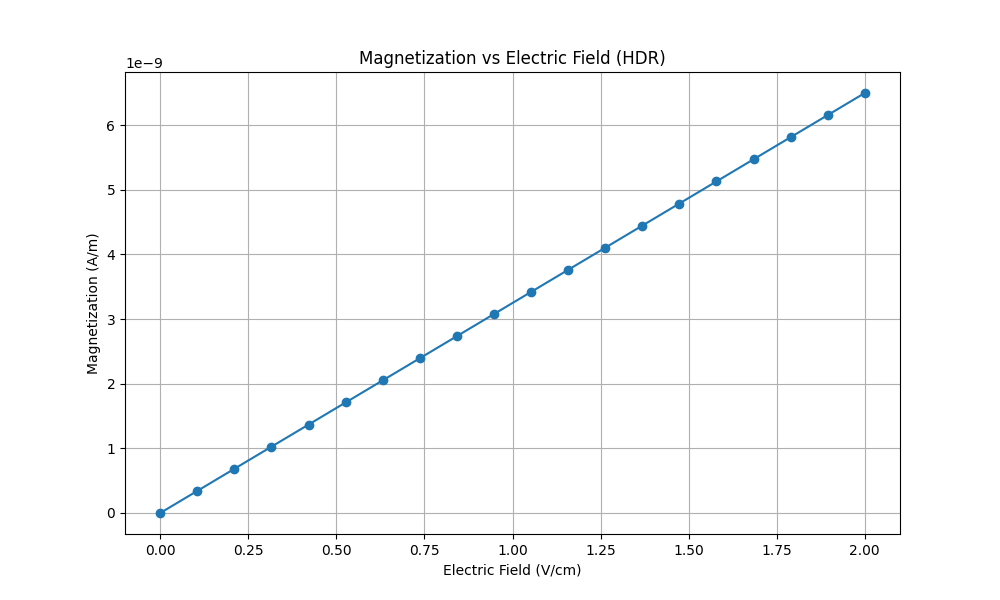
\includegraphics[width=1.0\textwidth]{data/mag_eField.png}
				\caption{magnetisation over electric field}
			\end{subfigure}
			\hfill
			\begin{subfigure}{0.49\textwidth}
				\centering
				
\includegraphics[width=1.0\textwidth]{data/mag_rashba.png}
				\caption{magnetisation over Rashba param. $\alpha$}
			\end{subfigure}
		\end{figure}
		}
		\uncover<1->{
		\begin{figure}
			\centering
			\begin{tikzpicture}[
				box/.style={
					rectangle, draw, rounded corners,
					minimum width=0.9cm, minimum height=0.2cm,
					align=center, fill=blue!5, font=\normalsize
				},
				graybox/.style={
					box, fill=gray!10
				},
				arrow/.style={->, thick},
				redbox/.style={
					rectangle, draw, rounded corners,
					minimum width=1.5cm, minimum height=0.6cm,
					align=center, fill=red!10, font=\scriptsize
				},
				bluebox/.style={
					box, fill=blue!10
				},
				smallbox/.style={
					rectangle, draw, rounded corners,
					minimum width=0.2cm, minimum height=0.1cm,
					align=center, fill=gray!10, font=\scriptsize
				},
				]
				
				\node[graybox] (input) {input};
				
				%first set
				\node (inf) at (input |- input) [graybox, xshift=1.9cm, yshift=0.0cm] {gather info};
				\draw [arrow, gray] (input) -- (inf);
				
				%				\node[graybox, right=0.3cm of input, yshift=0.4cm] (source) {find sources};
				%				\draw[arrow, gray] (input) -- (source);
				%				
				%				\node (info) at (source |- input) [bluebox, xshift=0cm,yshift=-0.4cm] {get info};
				%				\draw[arrow, red] (source) -- (info);
				
				%2. set
				\node (mod) at (source |- input) [graybox, xshift = 2.4cm, yshift=0.0cm] {build model};
				\draw [arrow, gray] (inf) -- (mod);
				
				%				\node (model) at (inf |- input) [smallbox, xshift=2.0cm, yshift=0.6cm] {model};
				%				\draw [arrow, gray] (inf) -- (model);
				%				
				%				\node (unit) at (model |- input) [smallbox, xshift=0cm, yshift=-0.0cm] {unit check};
				%				\draw [arrow, gray] (model) -- (unit);
				%				
				%				\node (param) at (unit |- unit) [bluebox, xshift= 0.0cm, yshift = -0.6cm] {param. sugg.};
				%				\draw [arrow, red] (unit) -- (param);
				
				%3. set
				%				\node (implement) at (mod |- input) [graybox, xshift = 2.7cm, yshift=0.0cm] {implementation};
				%				\draw [arrow, red] (param) -- (implement);
				
				\node (phyimpl) at (mod |- input) [bluebox, xshift=2.7cm, yshift=0.5cm] {physics implem.};
				\draw [arrow, red] (mod) -- (phyimpl);
				
				\node (corrimpl) at (phyimpl |- input) [bluebox, xshift=0cm, yshift=-0.5cm] {implem. check};
				\draw [arrow, red] (phyimpl) -- (corrimpl);
				
				%4. set
				%				\node (answer) at (phyimpl |- input) [graybox, xshift = 2.3 cm, yshift = 0cm] {answer};
				%				\draw [arrow, red] (corrimpl) -- (answer);
				
				%5. set
				\node (output) at (implement |- mod) [graybox, xshift = 2.5cm, yshift = 0.0cm] {output};
				\draw [arrow, red] (corrimpl) -- (output);
			\end{tikzpicture}
		\end{figure}
		}
	\end{frame}
	
	\section{next steps}
	
	\begin{frame}[c]{next steps}
		\uncover<1->{
		\begin{block}{benchmark the \enquote{physics-modelling-agent}}
			a method to measure the systems performance }
			\begin{itemize}
				\uncover<2->{\item use sciBench \autocite{wang2024scibench}: problems, solutions and execution script are open source; the problems are at high-school level}
				\uncover<3->{\item alternatively CritPt \autocite{critPtArx}\autocite{critptGit}: evaluation only via their servers, solutions are not public; problems are more difficult}
			\end{itemize}
		\end{block}
		\uncover<4->{
		\begin{exampleblock}{research the influence of (some of) the following aspects}}
			\begin{enumerate}
				\uncover<5->{\item agents temperature: which temperature maximizes performance?}
				\uncover<6->{\item LLM models: does performance increase with LLM complexity?}
				\uncover<7->{\item output variance: how consistent is the system over multiple runs?}
				\uncover<8->{\item execution time: how is it influenced by parameters?}
				\uncover<9->{\item sources: how does the number (and possibly type) of sources influence the systems results?}
			\end{enumerate}
		\end{exampleblock}
	\end{frame}
	
	\section{summary}
	
	\begin{frame}[c]{summary}		
		\begin{tikzpicture}[
			baseline=(current bounding box.center),
			stage/.style={
				rectangle, draw, rounded corners,
				minimum width=4.0cm, minimum height=0.6cm,
				align=center, fill=red!30, font=\large
			},
			sub/.style={
				rectangle, draw, rounded corners,
				minimum width=2.2cm, minimum height=0.5cm,
				align=center, fill=cyan!20, text=black, font=\small
			},
			info/.style={
				rectangle, draw, rounded corners,
				align=left, fill=green!20, font=\small, text width=2.7cm, inner sep=4pt
			},
			agent/.style={
				rectangle, draw, rounded corners,
				align=left, fill=green!20, font=\small, text width=3.7cm, inner sep=4pt
			},
			arrow/.style={->, thick},
			dashedarrow/.style={->, dashed, gray}
			]
			
			% ---------------- INPUT ----------------
			\node[stage] (input) {Input};
			\node[sub, right=0.69cm of input] (ffmr) {free form modelling request};
			\draw[arrow, gray] (input) -- (ffmr);
			
			\pause
			%%%%AGENT and TASK
			\node (task) at (input |- input) [info, xshift= 4.2cm, yshift=1.6cm] {
				\textbf{TASK}\\$\bullet$ description\\$\bullet$ expected output\\$\bullet$ agent
			};
			
			\node (agentbox) at (task |- task) [agent, xshift= 3.8cm, yshift=0.0cm] {
				\textbf{AGENT}\\$\bullet$ role, goal, backstory\\$\bullet$ LLM model, temperature\\$\bullet$ assigned tools
			};
			
			% ---------------- gather ----------------
			\pause
			\node[stage, below=0.6cm of input] (gather) {gather information};
			\draw[arrow, red] (input) -- (gather);
			
			\node[sub, right=0.69cm of gather] (arxiv) {arXiv search \& information extraction};
			\draw[arrow, gray] (gather) -- (arxiv);
			
			\pause
			% ---------------- model ----------------
			\node[stage, below=0.6cm of gather] (model) {suggest a model};
			\draw[arrow, red] (gather) -- (model);
			
			\node[sub, right=0.69cm of model] (modsug) {based on given information};
			\draw[arrow, gray] (model) -- (modsug);
			
			\pause
			% ---------------- unitcheck ----------------
			\node[stage, below=0.6cm of model] (unitCheck) {check \& correct units};
			\draw[arrow, red] (model) -- (unitCheck);
			
			\node[sub, right=0.69cm of unitCheck] (dimen) {dimensional analysis};
			\draw[arrow, gray] (unitCheck) -- (dimen);
			
			\pause
			% ---------------- implement -----------------
			
			\node[stage, below=0.6cm of unitCheck] (implement) {implement model};
			\draw[arrow, red] (unitCheck) -- (implement);
			
			\node[sub, right=0.69cm of implement] (python) {executable python code calculations};
			\draw[arrow, gray] (implement) -- (python);
		\end{tikzpicture}
	\end{frame}
	
	\begin{frame}[allowframebreaks]{sources}
		\printbibliography
	\end{frame}
\end{document}

% stokesche parameter